% ============================================================
% ViTool — RIVF 2026 CAMERA-READY (EDAS #1571323910)
% Compile with XeLaTeX. Put in the same folder:
%   fig1_heatmap_v6_v12.pdf, fig2_pareto_v6_v12.pdf   (eval/v6/paper_pack/)
% All numbers come from eval/v6/REPORT_v6.md (2026-11-13), v1.2 = main data.
%
% BEFORE UPLOAD:
%  [ ] \repourl: make the GitHub repo public and check the URL below.
%  [ ] \QwenVtwo: fill in when "m3_qwen27b_0shot_v12" finishes (TSR, 3 decimals);
%      until then the cell prints "pending" — do not upload with "pending".
%  [ ] EDAS author names must be First = "Duc Tai", Last = "Phan" and
%      First = "Trung Duc", Last = "Trinh Tran" (same as the PDF).
%  [ ] Run IEEE PDF eXpress, upload the certified PDF, sign the eCF.
% ============================================================
\documentclass[conference,a4paper]{IEEEtran}
\ifdefined\pdfminorversion\pdfminorversion=6\fi
\IEEEoverridecommandlockouts
\usepackage{cite}
\usepackage{amsmath,amssymb,amsfonts}
\usepackage{algorithm}
\usepackage{algorithmic}
\usepackage{graphicx}
\usepackage{textcomp}
\usepackage{xcolor}
\usepackage{booktabs}
\usepackage{url}
\usepackage{fontspec}
\setmainfont{TeX Gyre Termes}
\setmonofont{Latin Modern Mono}

\newcommand{\repourl}{\url{https://github.com/ductaip/budgetswitch}} % TODO check
\newcommand{\QwenVtwo}{pending} % TODO: Qwen3.8-27B 0-shot TSR on v1.2

\begin{document}
\special{pdf:minorversion 6}

\title{ViTool: An Executable Vietnamese Tool-Use Benchmark for Compute-Mode Allocation in Small Language Models}

\author{
\IEEEauthorblockN{Duc Tai Phan, Trung Duc Trinh Tran}
\IEEEauthorblockA{University of Transport Ho Chi Minh City, Vietnam\\
\texttt{dtai858@gmail.com}, \texttt{trinhtrantrungduc@gmail.com}}
}

\maketitle

\begin{abstract}
Tool-using language models are often given extra test-time compute, such as
reasoning, retrieval or deferral to a larger model, uniformly at every step. We
study whether a small language model needs it, using ViTool, an executable
Vietnamese tool-use benchmark of 373 trajectories over five domains and 36
deterministic tools, in which every gold trajectory is verified by execution
against a stateful environment. Building ViTool exposed a data-quality failure
that execution checks do not catch: in 54\% of the LLM-drafted trajectories,
the gold calls used argument values that the user never stated. We add a
grounding gate, repair the queries, and validate the repair with two
annotators. On the repaired benchmark, a LoRA-tuned 3B model that calls tools
directly reaches a task success rate of 0.688 and significantly outperforms
thinking (0.607), retrieval (0.527) and zero-shot deferral to gpt-oss-120b
(0.571). A per-step oracle reaches 0.804, but no deployable router we test
exceeds 0.705. Repairing the data alone raised task success by 0.14--0.25 for
every mode and more than doubled the routing headroom. We also document two
measurement pitfalls: assumed cost multipliers overstate the oracle's savings
over always-think about twofold compared with measured FLOPs (46.7\% vs
21.7\%), and teacher-forced step accuracy exceeds rollout step accuracy by 15
points while trajectory-level success is unaffected.
\end{abstract}

\begin{IEEEkeywords}
tool use, small language models, benchmark, Vietnamese NLP, test-time compute,
data quality
\end{IEEEkeywords}

\section{Introduction}
Tool-augmented language models increasingly spend test-time compute on
chain-of-thought, retrieval, or deferral to larger models~\cite{snell2024}.
This budget is usually spent uniformly, even though many steps of a tool-use
trajectory are simple calls. Work on overthinking and underthinking in
reasoning models~\cite{chen2024overthink,wang2025underthink,ttcsurvey2025}
suggests that extra compute can hurt on easy inputs and still be insufficient
on hard ones. For tool-use agents, and for Vietnamese in particular, this
trade-off has not been measured on an executable benchmark.

We introduce \textbf{ViTool}, an executable Vietnamese tool-use benchmark, and
use it to measure per-step compute-mode allocation in a 3B model. Building the
benchmark taught us as much as evaluating on it: an initial version passed
schema, placeholder, structure and execution checks as well as a
two-annotator review, yet more than half of its trajectories expected argument
values the user never gave. Models were penalised for not guessing them. We
report this failure, the gate that catches it, and how much it distorted every
conclusion of the study.\footnote{Data, environment, gates and harness:
\repourl}

Our contributions are:
\begin{itemize}
\item \textbf{ViTool v1.2}: 373 executable trajectories, 5 domains, 36
deterministic tools and five validation gates, including a new
\emph{grounding gate} that requires every gold argument to be stated by the
user, produced by an earlier tool call, or a schema default. The repair is
validated by two annotators.
\item \textbf{A controlled study of four compute modes} with measured cost
(tokens, FLOPs, latency). Direct calling is the best fixed mode; thinking,
retrieval and zero-shot deferral are significantly worse. A per-step oracle
shows +0.116 headroom that the routers we test do not capture.
\item \textbf{Three measurement findings}: ungrounded gold data lowered task
success by up to 0.25 and hid half of the routing headroom; assumed cost
multipliers inflate oracle savings about twofold; teacher-forced step accuracy
is inflated relative to rollout, but trajectory success is not.
\end{itemize}

\section{Related Work}
\textbf{Test-time compute.} Studies of reasoning models characterize
overthinking on easy inputs and underthinking on hard
ones~\cite{chen2024overthink,wang2025underthink,sui2025survey}, and surveys
review adaptive budget control~\cite{ttcsurvey2025}. We extend this lens from
free-form reasoning to tool-call trajectories, where each step has a discrete,
executable ground truth and compute can be measured per step.

\textbf{Tool-use benchmarks.} BFCL~\cite{bfcl2024} verifies calls by
abstract-syntax-tree matching; API-Bank~\cite{apibank2023} and
ToolLLM~\cite{toolbench2023} provide large API ecosystems, mostly in English.
ViTool verifies by execution against a stateful environment, targets
Vietnamese, and adds an explicit check that gold arguments are grounded in the
user's request.

\textbf{Vietnamese evaluation.} Vietnamese benchmarks cover QA, NLU and
instruction following~\cite{villmeval2024,viglue2024,crossing2024}; executable
tool use has not been covered.

\section{The ViTool Benchmark}

\subsection{Task, tools and environment}
A \emph{trajectory} pairs a Vietnamese user request with an ordered list of
gold tool calls; a \emph{step} is one call (tool name and arguments). The 36
tools cover banking, e-commerce, information retrieval, public services and
travel, and are deterministic functions over a shared \texttt{WorldState}, so
the same inputs always yield the same outputs and entity IDs. Difficulty is
structural: \emph{easy} = one call, \emph{medium} = several independent calls,
\emph{hard} = $\geq 3$ calls with at least one data dependency (e.g., a
\texttt{flight\_id} returned by \texttt{search\_flight} and consumed by
\texttt{book\_flight}). ViTool v1.2 has 373 trajectories (e-commerce 145,
travel 64, information retrieval 56, banking 55, public services 53).

\subsection{Construction and validation}
Trajectories were drafted by an LLM and filtered by the gates in
Algorithm~\ref{alg:gates}: schema validation, a placeholder gate,
a structure check, an executable gate that replays the trajectory and requires
a valid final state, and semantic de-duplication. The first release (v1, 375
trajectories) stopped there; a two-annotator review of 51 stratified
trajectories accepted 45 and asked for minor edits on 6 (raw agreement 92.2\%,
Gwet's AC1 $=0.91$~\cite{gwet2008}). We provide a datasheet~\cite{datasheets2021}.

\begin{algorithm}[t]
\caption{ViTool trajectory validation (v1.2)}
\label{alg:gates}
\begin{algorithmic}[1]
\REQUIRE draft $\tau=(q,[s_1,\dots,s_k])$; catalog $C$; environment $\mathcal{E}$
\STATE \textbf{Gate 1 (schema):} reject if any $s_i$ violates $C$
\STATE \textbf{Gate 1.5 (placeholder):} reject unresolved or empty values
\STATE \textbf{Structure:} reject if declared tier $\neq$ structural tier
\STATE resolve dependent IDs from $\mathcal{E}$'s realized outputs
\STATE \textbf{Gate 2 (executable):} run $[s_1,\dots,s_k]$ on $\mathcal{E}$;
reject on error or invalid final state
\STATE \textbf{Gate G3 (grounding):} reject unless every argument value of every
$s_i$ is stated in $q$ (after normalization), returned by an earlier step, or a
schema default
\STATE semantic dedup (multilingual-e5, $\cos>0.93$)
\RETURN $\tau$
\end{algorithmic}
\end{algorithm}

\subsection{Grounding audit and repair}
\label{sec:grounding}
While analysing failures we found gold arguments that no model could produce:
for example, an account number \texttt{1234567890} or a payment method that
appears nowhere in the request. Gate G3 normalizes Vietnamese dates, numbers and
money (``500.000đ'', ``2 triệu đồng''), maps a small lexicon (currencies,
languages, cities), and, for enumerated arguments, accepts a value only when the
request names it literally or through a Vietnamese phrase table (e.g.,
``thanh toán khi nhận hàng'' $\rightarrow$ \texttt{cod}).

\textbf{Validation of the gate.} Two authors independently labelled 60
argument values (40 flagged, 20 not; stratified). Agreement was 86.7\%
(Cohen's $\kappa=0.76$); after adjudicating 8 items, G3 matched all 60 labels.

\textbf{Extent.} Under G3, 203 of the 375 v1 trajectories (54\%) contain at
least one ungrounded value, including 63 of the 112 evaluation trajectories and at
least 39 of the 43 hard ones. The most frequent are quantities, price caps, passenger
names, voucher codes, payment methods and platforms. Many are recurring
``conventional'' values (e.g., \texttt{1234567890}) that also occur in the
training split.

\textbf{Repair.} We rewrote only the \emph{request} of each failing trajectory
so that it states the missing values, leaving gold calls, tier, domain and split
unchanged. The rewriter (gpt-oss-20b, temperature 0) received the missing values
and a Vietnamese wording hint for enumerated codes; a rewrite was accepted only
if all gates passed and at least 70\% of the original words were kept. Repair
ran in two rounds (v1.1: non-enumerated values; v1.2: enumerated choices). Two
train trajectories with placeholder gold values were removed. All 373 remaining
trajectories pass every gate. Rewrites are small: in the second round the
median edit is 30 characters and 91\% are pure insertions.

\textbf{Human checks of the repair.} On 50 random rewrites, both annotators
judged meaning preserved in 50/50 cases; none was rated unnatural (mean
naturalness 2.48 and 2.54 on a 1--3 scale, weighted $\kappa=0.16$ on the
2-vs-3 distinction). In 30 random v1.1 trajectories the annotators still found
3 and 4 unstated values, all enumerated choices, which motivated round two; in
20 random v1.2 trajectories both found none (Wilson upper bound 0.16).

\section{Experimental Setup}

\subsection{Compute modes}
The local model is Qwen2.5-3B-Instruct~\cite{qwen25} (4-bit) with a
LoRA~\cite{lora2021} adapter trained on the v1 training split (263
trajectories, 719 steps). We evaluate four modes:
\textbf{M0} (fast): direct tool call;
\textbf{M1} (think): a short chain of thought, then the call;
\textbf{M2} (search): retrieve a tool subset with multilingual
e5~\cite{e5multi2024}, think, then call;
\textbf{M3} (defer): zero-shot gpt-oss-120b via the Groq API, a different
model family from the v1 data generator. Retraining the adapter on the
repaired training split did not change any mode significantly (M0:
$\Delta=-0.036$, $p=0.31$), so we keep the original adapter.

\subsection{Metrics}
All results are on 112 held-out trajectories (284 steps; 43 easy, 26 medium,
43 hard). \textbf{TSR} (task success rate, main metric) counts a trajectory as
solved when every call strictly matches gold and the executed calls reproduce
the gold final state. \textbf{SSR} (step success rate) is reported in two
settings: \emph{teacher-forced} (SSR$_\text{tf}$), where every step sees the
gold history, and \emph{rollout} (SSR$_\text{ro}$), where the model sees its
own earlier calls and observations. Decoding is greedy (seed 42). We report
Wilson 95\% intervals, McNemar tests on steps, and paired bootstrap tests
(10k resamples by trajectory) on TSR.

\subsection{Cost models}
Besides assumed relative multipliers (1/3/5/15 for M0--M3), a common proxy,
we measure per step: prompt and completion tokens, latency, and FLOPs
$\approx 2N_\text{active}(\text{prompt}+\text{completion})$, with
$N_\text{active}=3.09$B for the 3B model, 5.1B for gpt-oss-120b (mixture of
experts), and the e5 encoder added for M2.

\subsection{Oracle and routers}
The \emph{oracle} selects, per step, the cheapest mode whose call is correct
(the cheapest mode if none is). It uses outcomes unavailable at inference and
is an upper bound, not a policy. Deployable routers: a random router; a length
router (query-length terciles $\rightarrow$ M0/M1/M2); an error cascade that
runs M0 and escalates to M1 or M3 when M0's call fails to parse or execute; and
a learned pre-generation router (logistic regression on character n-grams and
step position, 5-fold cross-validation grouped by trajectory) that maximizes
predicted success minus $\lambda\cdot$cost. A semi-oracle escalates by the gold
difficulty tier.

\section{Results}

\begin{table}[t]
\caption{Modes on ViTool v1.2 (112 trajectories, 284 steps). TSR with Wilson
95\% CI; SSR teacher-forced (tf) and rollout (ro); cost per step relative to
M0 (M0: 562 tokens, $3.5\times10^{12}$ FLOPs).}
\label{tab:main}
\centering
\footnotesize
\setlength{\tabcolsep}{2.6pt}
\begin{tabular}{lccccccc}
\toprule
Mode & TSR & SSR$_\text{tf}$ & SSR$_\text{ro}$ & easy & med. & hard & FLOPs \\
\midrule
M0 fast   & \textbf{0.688} {\scriptsize[.60,.77]} & \textbf{0.873} & \textbf{0.722} & \textbf{1.00} & \textbf{0.62} & \textbf{0.42} & 1.00$\times$ \\
M1 think  & 0.607 {\scriptsize[.51,.69]} & 0.824 & 0.665 & 0.91 & 0.46 & 0.40 & 1.09$\times$ \\
M2 search & 0.527 {\scriptsize[.43,.62]} & 0.768 & 0.532 & 0.86 & 0.46 & 0.23 & 0.66$\times$ \\
M3 defer  & 0.571 {\scriptsize[.48,.66]} & 0.757 & -- & 0.88 & 0.54 & 0.28 & 4.28$\times$ \\
\midrule
Oracle    & 0.804 {\scriptsize[.72,.87]} & 0.944 & -- & 1.00 & 0.81 & 0.60 & -- \\
\bottomrule
\end{tabular}
\end{table}

\begin{figure*}[t]
\centering
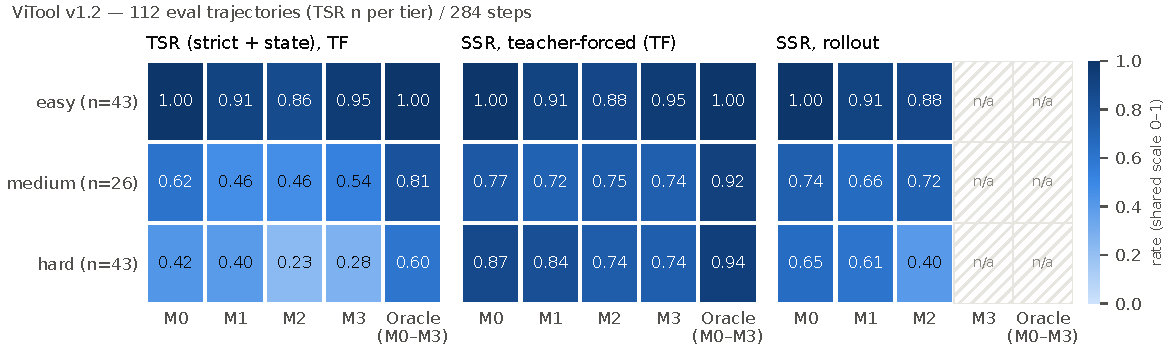
\includegraphics[width=\textwidth]{fig1_heatmap_v6_v12.pdf}
\caption{ViTool v1.2 by difficulty tier and mode: TSR (left), teacher-forced
SSR (middle) and rollout SSR (right), on one color scale. M3 and the oracle are
not run in rollout.}
\label{fig:heatmap}
\end{figure*}

\subsection{Direct calling is the best fixed mode}
Table~\ref{tab:main} and Fig.~\ref{fig:heatmap} show that M0 is the best fixed
mode on TSR in every tier, and best or tied best in four of five domains (in
public services M3 scores 0.875 vs.\ 0.812). On trajectory
success it is significantly better than thinking ($-0.080$, $p=0.019$),
retrieval ($-0.161$, $p<0.001$) and deferral ($-0.116$, $p=0.016$); the step
level agrees (McNemar: M0 wins 19 vs.\ 5 steps against M1, 50 vs.\ 17 against
M3). On easy requests M0 solves all 43, while think and search lose 4--6:
extra reasoning before a one-call request mostly adds opportunities to change a
correct call. Retrieval is the weakest local mode: with 36 tools the full
catalog fits in context, and filtering it removes the right tool more often
than it helps. E-commerce, with the longest dependency chains, remains the
hardest domain (M0 TSR 0.48 vs.\ 0.74--0.94 elsewhere).

\subsection{Deferral to larger models}
\label{sec:defer}
Zero-shot gpt-oss-120b (M3) reaches 0.571 on v1.2 at $4.3\times$ M0's FLOPs.
Table~\ref{tab:defer} adds variants run on v1.1 (before the enumerated-value
repair). Three demonstrations raise gpt-oss to 0.571, and a dense 27B model
(Qwen3.8-27B, zero-shot) reaches 0.625, above the 3B model's 0.598 on the same
data, but at about $22\times$ its FLOPs and $4.5\times$ gpt-oss's API price.
Larger models therefore can help, at a cost far above that of the routing
gains below. Three repeated M3 runs varied by $\pm0.016$ TSR.

\begin{table}[t]
\caption{Deferral variants (TSR). FLOPs per step relative to M0 on the same
data. v1.1 = ViTool before the enumerated-value repair.}
\label{tab:defer}
\centering
\footnotesize
\setlength{\tabcolsep}{4pt}
\begin{tabular}{llccc}
\toprule
Data & Model & TSR & FLOPs & USD/284 steps \\
\midrule
v1.1 & 3B LoRA, M0 (reference) & 0.598 & 1.0$\times$ & -- \\
v1.1 & gpt-oss-120b, 0-shot (3 runs) & 0.518$\pm$0.016 & 4.4$\times$ & 0.079 \\
v1.1 & gpt-oss-120b, 3-shot & 0.571 & 5.5$\times$ & 0.096 \\
v1.1 & Qwen3.8-27B, 0-shot & 0.625 & 22$\times$ & 0.353 \\
\midrule
v1.2 & 3B LoRA, M0 (reference) & 0.688 & 1.0$\times$ & -- \\
v1.2 & gpt-oss-120b, 0-shot & 0.571 & 4.3$\times$ & 0.078 \\
v1.2 & Qwen3.8-27B, 0-shot & \QwenVtwo & 22$\times$ & -- \\
\bottomrule
\end{tabular}
\end{table}

\subsection{Effect of ungrounded gold data}
Table~\ref{tab:versions} evaluates the same models on the same 112
trajectories before and after repair. Every mode gains 0.14--0.25 TSR
(paired bootstrap, $p<0.001$ from v1 to v1.2), almost all of it on medium and
hard tasks: hard-tier TSR of M0 rises from 0.05 to 0.42. On v1, the failures
were mostly not model errors but requests that lacked the expected value. The
repair also changes the conclusions. On v1 the modes were statistically
indistinguishable on TSR and the oracle exceeded the best fixed mode by only
0.053; on v1.2, M0 is significantly best and the headroom is 0.116. The only
mode that asked the user for missing information on v1 was M3 (7 of 284 steps,
all on ungrounded steps), behavior that the strict metric counted as failure.

\begin{table}[t]
\caption{TSR on the same 112 trajectories before (v1) and after the two repair
rounds (v1.1, v1.2); same adapter and decoding.}
\label{tab:versions}
\centering
\footnotesize
\begin{tabular}{lccc}
\toprule
& v1 & v1.1 & v1.2 \\
\midrule
M0 fast   & 0.438 & 0.598 & \textbf{0.688} \\
M1 think  & 0.420 & 0.554 & 0.607 \\
M2 search & 0.384 & 0.509 & 0.527 \\
M3 defer  & 0.393 & 0.527 & 0.571 \\
Oracle    & 0.491 & 0.732 & 0.804 \\
\midrule
M0, hard tier & 0.046 & 0.233 & 0.419 \\
Oracle $-$ best fixed mode & 0.053 & 0.134 & 0.116 \\
\bottomrule
\end{tabular}
\end{table}

\subsection{Teacher-forced vs.\ rollout evaluation}
Teacher forcing inflates step accuracy: M0's SSR is 0.873 teacher-forced and
0.722 in rollout (v1: 0.588 vs.\ 0.468), because after a wrong call the gold
history hides the error from later steps. Trajectory success is unaffected
(M0 0.688 vs.\ 0.679; M1 0.607 in both): a trajectory is solved only if every
call is correct, and then the model's own history equals the gold history.
Step accuracy should therefore always state its history setting; TSR does not
need to.

\section{Routing and Cost}

\begin{table}[t]
\caption{Policies on ViTool v1.2. Cost per step relative to always-M0.}
\label{tab:routers}
\centering
\footnotesize
\setlength{\tabcolsep}{3.5pt}
\begin{tabular}{lcccc}
\toprule
Policy & TSR & Assumed & Tokens & FLOPs \\
\midrule
Fixed M0 & 0.688 & 1.00 & 1.00 & 1.00 \\
Fixed M1 & 0.607 & 3.00 & 1.09 & 1.09 \\
Fixed M2 & 0.527 & 5.00 & 0.65 & 0.66 \\
Fixed M3 & 0.571 & 15.00 & 2.59 & 4.28 \\
\midrule
Random & 0.591 & 6.00 & 1.33 & 1.76 \\
Length router & 0.562 & 3.77 & 0.84 & 0.84 \\
Cascade M0$\rightarrow$M1 on error & 0.696 & 1.01 & 1.00 & 1.00 \\
Learned router (CV, best) & 0.705 & 2.04 & 1.02 & 1.09 \\
Gold-tier escalation (semi-oracle) & 0.598 & 10.64 & 2.10 & 3.27 \\
\midrule
Oracle (cheapest correct) & 0.804 & 1.60 & 0.79 & 0.86 \\
\bottomrule
\end{tabular}
\end{table}

\begin{figure}[t]
\centering
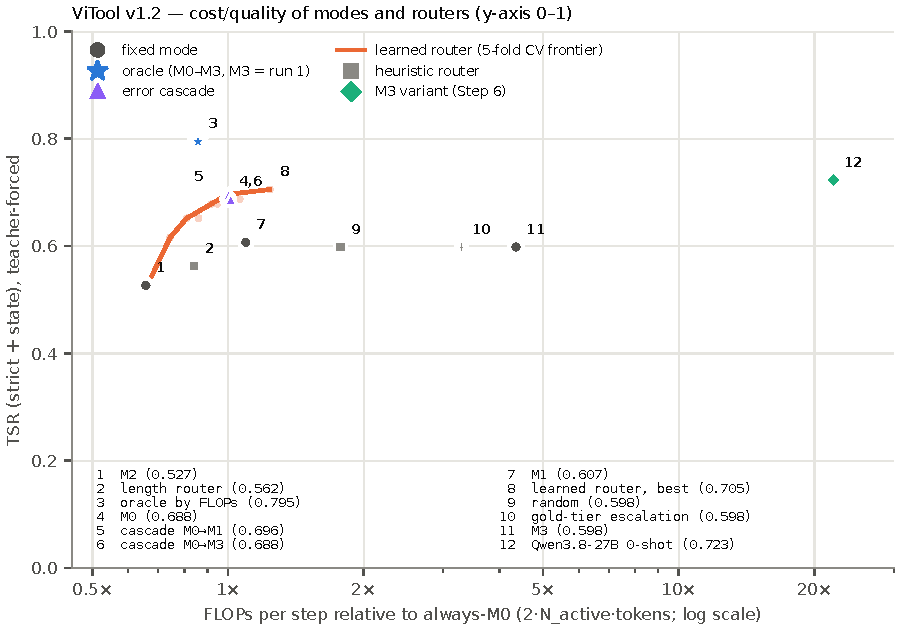
\includegraphics[width=\columnwidth]{fig2_pareto_v6_v12.pdf}
\caption{TSR vs.\ measured FLOPs per step (relative to always-M0, log scale)
on ViTool v1.2. Points are numbered; the oracle here selects by FLOPs (TSR
0.795).}
\label{fig:pareto}
\end{figure}

\textbf{Measured cost changes the size of the savings.} Under the assumed
multipliers the oracle costs 46.7\% less than always-think (M1) while scoring
0.197 higher. Under measured costs the saving is 27.9\% (tokens) and 21.7\%
(FLOPs): think is only 1.09$\times$ M0, because its reasoning is short, and
search is the \emph{cheapest} mode (0.66$\times$), because the retrieved tool
subset shortens the prompt. The same holds on v1 (51.2\% assumed vs.\ 16.9\%
FLOPs). Measured latency on our hardware (two T4 GPUs; medians M0 6.0 s,
M1 9.9 s, M2 8.3 s) and API latency for M3 (0.9 s, hardware not disclosed)
are not comparable across modes and are not used for routing.

\textbf{Routers do not capture the headroom.} No deployable router
(Table~\ref{tab:routers}, Fig.~\ref{fig:pareto}) improves on M0 by more than
0.017 TSR (two trajectories). The learned router reaches 0.705 at nearly M0's cost; its per-mode
success classifiers reach AUC of only 0.56--0.62 once requests are grounded
(0.74--0.80 on v1, where ``the request lacks a value'' was an easy failure
signal). The error cascade triggers on 0.4\% of steps, because almost all of
M0's wrong calls are well-formed and executable; it gains 0.009. The oracle's
0.116 margin comes from steps where a different mode makes a different but
correct choice, and pre-generation features do not predict which.

\section{Limitations}
\label{sec:limitations}
\textbf{Scope.} The tools are deterministic mocks, so results characterize
allocation behavior rather than live APIs. The main study uses one 3B backbone;
the evaluation set has 112 trajectories, so differences of a few points are not
significant. E-commerce provides 44 of 112 trajectories; we report
domain-level results alongside the aggregates.
\textbf{Data repair.} Requests were rewritten by an LLM from the same family as
the deferral model (gpt-oss), with only minimal insertions accepted and human
checks reported above. The repair also makes some requests longer and more
list-like. Gold calls were not re-derived, so oddities in the original gold
(e.g., an unrelated extra step) remain; annotators flagged 4 of 50.
\textbf{Metric.} TSR uses strict argument matching plus a final-state check. A
relaxed variant that accepted normalized or execution-equivalent calls was
correct in only 1 of 20 manually checked cases, because the mock environment
ignores optional arguments, so we keep the strict metric.
\textbf{Deferral.} The small modes are fine-tuned on ViTool, the large models
are not; our deferral results describe off-the-shelf deferral, not an adapted
large model. The think mode uses a short synthetic template, not elicited
long reasoning.

\section{Conclusion}
ViTool shows that, for a fine-tuned 3B tool caller on grounded Vietnamese
requests, spending more compute per step does not help on average: direct
calling beats thinking, retrieval and zero-shot deferral. A per-step oracle
still gains 0.116 TSR at lower cost, but the routers we test do not find it,
and measured costs make the potential saving about half as large as assumed
multipliers suggest. The largest effect in our study came from the data:
ungrounded gold arguments in LLM-drafted trajectories passed execution-based
validation and human review, lowered measured success by up to 0.25, and hid
half of the routing headroom. We recommend a grounding gate for synthetic
tool-use data and release ViTool v1.2 with its gates, environment, per-step
outcomes and harness to support learned routing for efficient tool use.

\section*{Acknowledgment}
Experiments used free GPU quota from Kaggle and the Groq API.

\begin{thebibliography}{00}

\bibitem{chen2024overthink}
X. Chen \emph{et al.}, ``Do Not Think That Much for 2+3=? On the Overthinking
of o1-Like LLMs,'' arXiv:2412.21187, 2024.

\bibitem{wang2025underthink}
Y. Wang \emph{et al.}, ``Thoughts Are All Over the Place: On the Underthinking
of o1-Like LLMs,'' arXiv:2501.18585, 2025.

\bibitem{sui2025survey}
Y. Sui \emph{et al.}, ``Stop Overthinking: A Survey on Efficient Reasoning for
Large Language Models,'' arXiv:2503.16419, 2025.

\bibitem{ttcsurvey2025}
M. A. Alomrani \emph{et al.}, ``Reasoning on a Budget: A Survey of Adaptive
and Controllable Test-Time Compute in LLMs,'' arXiv:2507.02076, 2025.

\bibitem{snell2024}
C. Snell, J. Lee, K. Xu, and A. Kumar, ``Scaling LLM Test-Time Compute
Optimally Can Be More Effective than Scaling Model Parameters,''
arXiv:2408.03314, 2024.

\bibitem{bfcl2024}
F. Yan \emph{et al.}, ``Berkeley Function Calling Leaderboard,'' 2024.
[Online]. Available: \url{https://gorilla.cs.berkeley.edu/leaderboard.html}

\bibitem{apibank2023}
M. Li \emph{et al.}, ``API-Bank: A Comprehensive Benchmark for Tool-Augmented
LLMs,'' in \emph{Proc. EMNLP}, 2023.

\bibitem{toolbench2023}
Y. Qin \emph{et al.}, ``ToolLLM: Facilitating Large Language Models to Master
16000+ Real-World APIs,'' arXiv:2307.16789, 2023.

\bibitem{villmeval2024}
T.-H. Nguyen, A.-C. Le, and V.-C. Nguyen, ``ViLLM-Eval: A Comprehensive
Evaluation Suite for Vietnamese Large Language Models,'' arXiv:2404.11086,
2024.

\bibitem{viglue2024}
M. Tran \emph{et al.}, ``ViGLUE: A Vietnamese General Language Understanding
Benchmark and Analysis,'' in \emph{Findings of NAACL}, 2024.

\bibitem{crossing2024}
S. Truong \emph{et al.}, ``Crossing Linguistic Horizons: Finetuning and
Comprehensive Evaluation of Vietnamese Large Language Models,''
arXiv:2403.02715, 2024.

\bibitem{qwen25}
Qwen Team, ``Qwen2.5 Technical Report,'' arXiv:2412.15115, 2024.

\bibitem{lora2021}
E. J. Hu \emph{et al.}, ``LoRA: Low-Rank Adaptation of Large Language Models,''
arXiv:2106.09685, 2021.

\bibitem{e5multi2024}
L. Wang \emph{et al.}, ``Multilingual E5 Text Embeddings: A Technical Report,''
arXiv:2402.05672, 2024.

\bibitem{datasheets2021}
T. Gebru \emph{et al.}, ``Datasheets for Datasets,'' \emph{Commun. ACM},
vol.~64, no.~12, pp.~86--92, 2021.

\bibitem{gwet2008}
K. L. Gwet, ``Computing Inter-Rater Reliability and Its Variance in the
Presence of High Agreement,'' \emph{British J. Math. Stat. Psychol.},
vol.~61, no.~1, pp.~29--48, 2008.

\end{thebibliography}

\end{document}